\documentclass[
% opciók nélkül: egyoldalas nyomtatás, elektronikus verzió
% twoside,     % kétoldalas nyomtatás
% tocnopagenum,% oldalszámozás a tartalomjegyzék után kezdődik
]{thesis-ekf}
\usepackage[T1]{fontenc}
\PassOptionsToPackage{defaults=hu-min}{magyar.ldf}
\usepackage[magyar]{babel}
\usepackage{mathtools,amssymb,amsthm,pdfpages}
\footnotestyle{rule=fourth}

\newtheorem{tetel}{Tétel}[chapter]
\theoremstyle{definition}
\newtheorem{definicio}[tetel]{Definíció}
\theoremstyle{remark}
\newtheorem{megjegyzes}[tetel]{Megjegyzés}

\begin{document}
\institute{Matematikai és Informatikai Intézet}
\title{Jelenlétkövető alkalmazás fejlesztése}
\author{Györkis Tamás\\Programtervező informatikus BSc}
\supervisor{Dr. Király Roland\\Egyetemi docens}
\city{Eger}
\date{2024}
\maketitle
\tableofcontents

\chapter*{Bevezetés}
\addcontentsline{toc}{chapter}{Bevezetés}
Amikor szakdolgozati témaválasztás előtt álltam, sokat gondolkoztam a témán. Mindenképpen egy olyan alkalmazást szerettem volna elkészíteni, mely ténylegesen hasznos is lehet. Egyetemi éveim alatt demonstrátorként tanítottam több féléven át az egyetemen, és innen jött a felismerés, hogy jó lenne, ha a hallgatók jelenlétét, hiányzásait ne táblázatokban kelljen vezetni, hanem egy külön eszköz legyen rá készítve. Innen származik az alkalmazás ötlete.

A megvalósítás során törekedtem arra, hogy egy jól átlátható, ergonomikus weboldalt készítsek, amit -- esetleges kisebb módosításokkal -- ne csak egyetemi környezetben lehessen használni. Ezekből kifolyólag egy webalkalmazást készítettem, mivel ezt a legegyszerűbb elérni, hiszen csak egy webböngésző szükséges hozzá. A tanulók és tanárok által használt oldalak reszponzívan lettek elkészítve, ezáltal biztosítva, hogy mobiltelefonon is használni lehessen. Illetve az alkalmazás PWA funkciókkal rendelkezik, aminek jelentőségére később térek ki, de előjáróban annyit érdemes megemlíteni róla, hogy lehetővé teszi a weboldal alkalmazásként való telepítését számítógép és telefon esetén is, ezáltal egy rendes alkalmazás érzését keltve.

A megvalósításhoz a Laravel keretrendszert használtam, mely egy PHP alapú, MVC keretrendszer, amivel tanulmányaim során találkoztam, és egyből megkedveltem. Nem titkolt célom a szakdolgozatommal, hogy bemutassam, hogy a mai, JavaScript preferált világban, továbbra is lehetséges modern, a mai kort kielégítő weboldalt készíteni PHP segítségével, amihez különböző csomagokat alkalmaztam, amiknek működését, illetve egymással való működését a későbbiekben fogom kifejteni.

\chapter{Alkalmazás bemutatása}
\section{Adatbázis}
\section{Általános funkciók, információk}
\section{Adminisztrátori nézet, funkciók}
\section{Tanári nézet, funkciók}
\section{Hallgatói nézet, funkciók}

\chapter{Felhasznált technológiák, csomagok}

\section{Laravel}
\subsection{Keretrendszer alapjai}
\subsection{MVC architektúra}
\subsection{Eloquent ORM}
\subsection{Blade templating engine}
\subsection{Laravel Fortify}
\subsection{Események, queue}
\subsection{Email küldés}

\section{LiveWire}
\subsection{Ismertető, a csomag működése}
\subsection{LiveWire és SPA}
\subsection{Komponensek és data binding}
\subsection{Események, lapozás}
\subsection{Alpine.js: LiveWire és JavaScript kapcsolata}
\subsection{WireToast: LiveWire alapú értesítések}

\section{Websocket és Pusher szerviz}
\subsection{Websocket jelentősége}
\subsection{Pusher}
\subsection{Websocket integrálása a keretrendszerbe}
\subsection{Csatornák, események létrehozása}
\subsection{Események fogadása JavaScript, LiveWire esetén}

\section{QR-kód generálás}

\section{Naptár - FullCalendar.js}
\subsection{Beállításai}
\subsection{Kapcsolat a keretrendszerrel LiveWire segítségével}

\section{Diagramok - Chart.js}
\subsection{Beállításai}
\subsection{Kapcsolat a keretrendszerrel LiveWire segítségével}

\section{Progressive Web Apps}
\subsection{A PWA jelentése, jelentősége}
\subsection{Laravel PWA csomag}
\subsection{A manifest fájl}
\subsection{Service Worker}

\chapter{Az alkalmazás tesztelése}
\section{Manuális tesztelés}
\section{Automatizált tesztelés}
\section{Terheléses tesztelés}

\chapter{Alkalmazás telepítése}
\section{Laravel Forge}
\section{Kézi telepítés lépései}

\chapter*{Összegzés}
\addcontentsline{toc}{chapter}{Összegzés}

\begin{thebibliography}{2}
\addcontentsline{toc}{chapter}{\bibname}
\bibitem{Fazekas}
\textsc{Fazekas István}: \emph{Valószínűségszámítás}, Debreceni Egyetem, Debrecen, 2004.
\bibitem{Tomacs}
\textsc{Tómács Tibor}: \emph{A valószínűségszámítás alapjai}, Líceum Kiadó, Eger, 2005.
\end{thebibliography}

% Aláírt, szkennelt nyilatkozat beillesztése a szakdolgozat végére
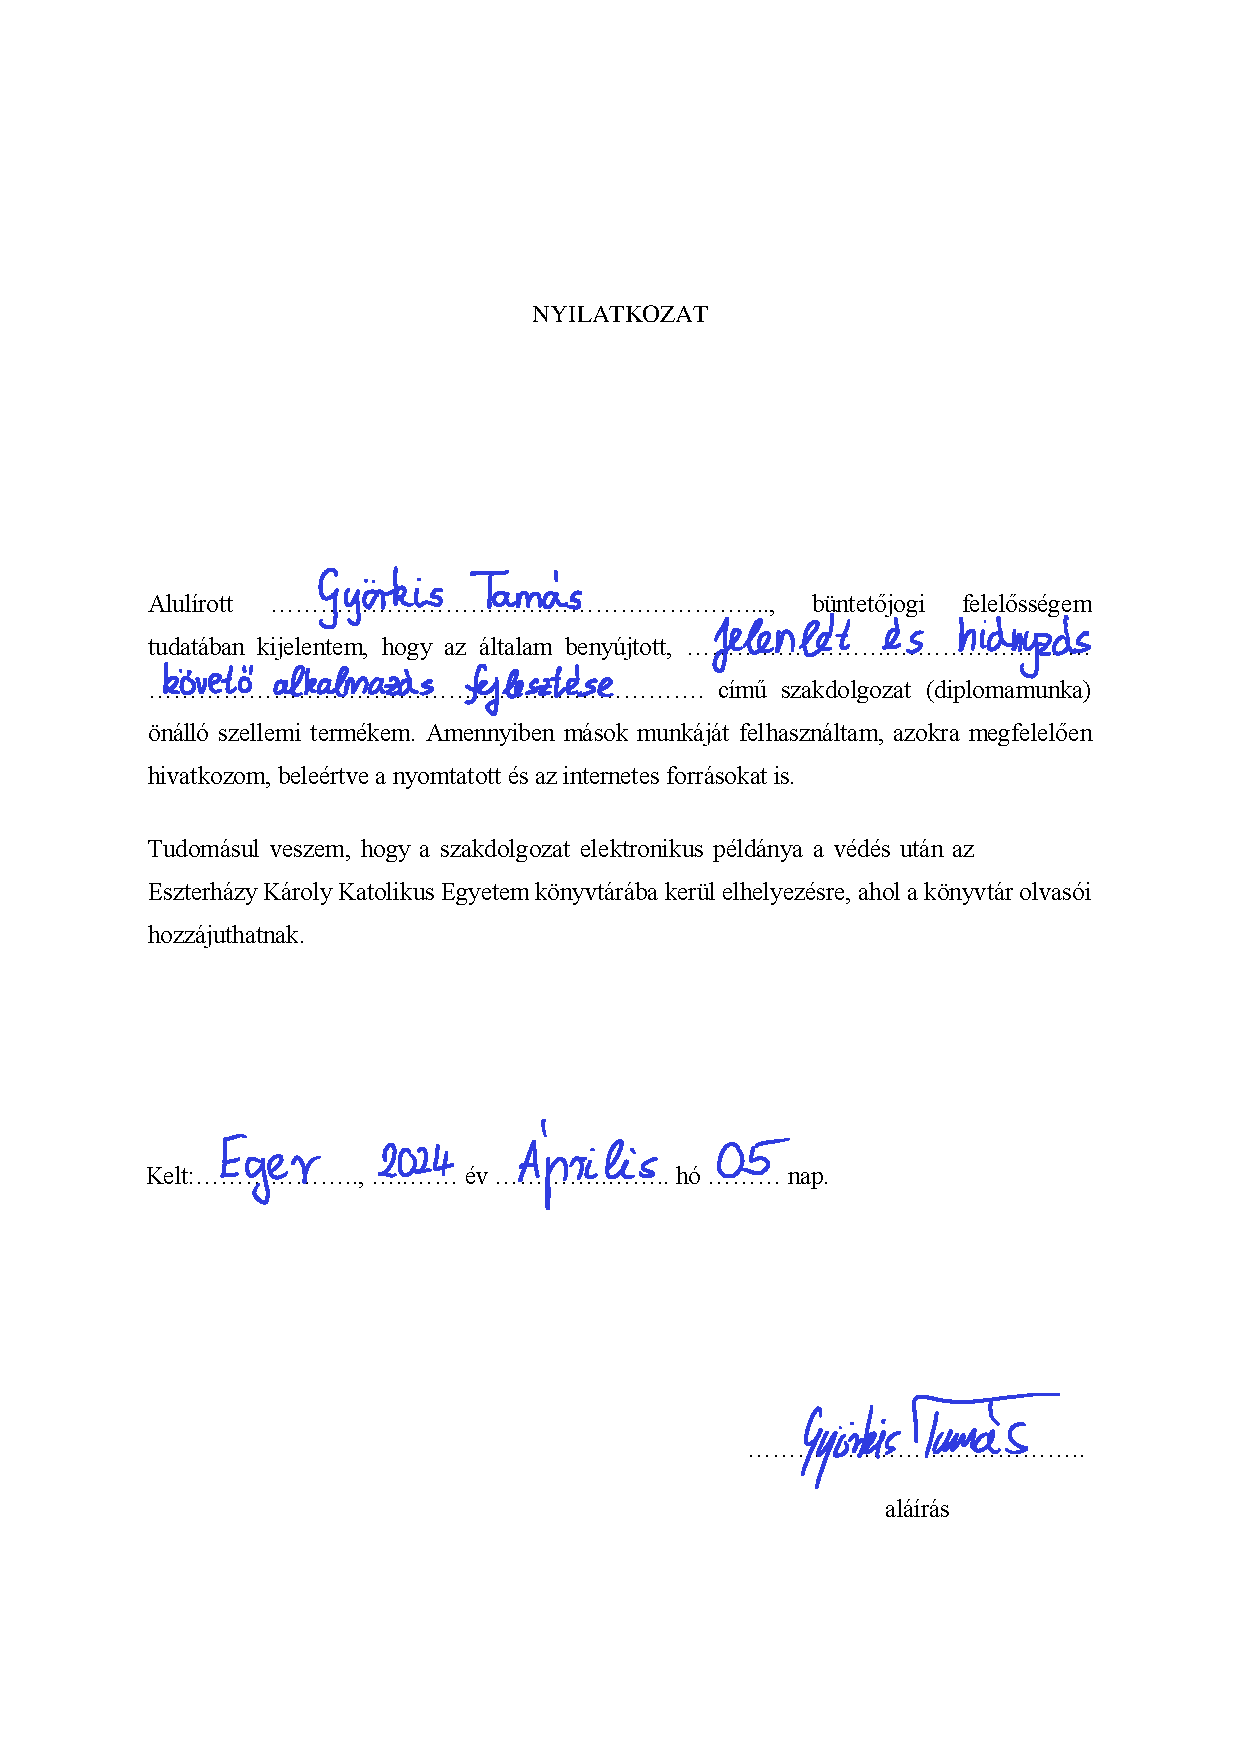
\includepdf{nyilatkozat.pdf}
\end{document}